\documentclass[20pt,a0paper,blockverticalspace=20mm]{tikzposter}

\usepackage[american]{babel}
\usepackage[utf8]{inputenc}
\usepackage[T1]{fontenc}
\usepackage{amsmath,amssymb}
\usepackage{tikzsymbols}
\usepackage{wrapfig,graphicx}
\usepackage{tikz}
\usetikzlibrary{matrix,arrows,arrows.meta,positioning}
\tikzset{>/.tip={Computer Modern Rightarrow[scale=2,line width=1pt]}}
\tikzset{|/.tip={Bar[scale=2,line width=1pt]}}
\tikzset{c_/.tip={Hooks[scale=2,line width=1pt,right]}}
\tikzset{c^/.tip={Hooks[scale=2,line width=1pt,left]}}

\def\Q {\ensuremath{\mathbb{Q}}}
\def\Z {\ensuremath{\mathbb{Z}}}
\def\F {\ensuremath{\mathbb{F}}}
\def\Tr {\ensuremath{\mathrm{Tr}}}
\def\M {\ensuremath{\mathsf{M}}}
\def\tildO {\ensuremath{\mathrm{\tilde{O}}}}

\DeclareMathOperator{\Gal}{Gal}
\DeclareMathOperator{\ord}{ord}

\renewcommand{\paragraph}[1]{\smallskip\textbf{#1}}
\newcommand{\secblock}[1]{\block[]{}{\huge\sc #1}}

\title{Computing isomorphisms and embeddings of finite fields}
\author{Ludovic Brieulle\footnotemark[1], Luca De Feo\footnotemark[1],
  Javad Doliskani\footnotemark[2], Jean-Pierre Flori\footnotemark[3],
  Éric Schost\footnotemark[2]} \institute{\footnotemark[1]Université
  de Versailles -- Saint-Quentin-en-Yvelines,
  \footnotemark[2]University of Western Ontario,
  \footnotemark[3]Agence Nationale de Sécurité des Systèmes
  d'Information}

\usetheme{Desert}

\definecolorpalette{UVSQ}{
    \definecolor{colorOne}{RGB}{255,255,255}
    \definecolor{colorTwo}{RGB}{0,146,187}
    %\definecolor{colorThree}{RGB}{119,173,28}
}
\colorlet{alert}{red}
\usecolorstyle[colorPalette=UVSQ]{Sweden}

\definetitlestyle{WLogos}{
    width=\paperwidth, roundedcorners=0, linewidth=0pt, innersep=1.5cm,
    titletotopverticalspace=0mm, titletoblockverticalspace=20mm,
    titlegraphictotitledistance=10pt, titletextscale=1
}{
   \draw[draw=none, bottom color=titlebgcolor, top color=framecolor,opacity=0.9]%
   (\titleposleft,\titleposbottom) rectangle (\titleposright,\titlepostop); %
   \draw
   (\titleposleft,0.75*\titlepostop+0.25*\titleposbottom)
   node[anchor=west]{\includegraphics[width=15em]{uvsq-logo-cmjn}}
   (\titleposright-1em,0.75\titlepostop+0.25*\titleposbottom)
   node[anchor=east]{\includegraphics[width=15em]{western}}
   (\titleposleft+1em,\titleposbottom+1em)
   node[anchor=south west]{\includegraphics[height=5em]{Anssi}}
   (\titleposright-1em,\titleposbottom+1em)
   node[anchor=south east]{\includegraphics[height=5em]{Anssi}};
}
\usetitlestyle{WLogos}

\pgfmathsetseed{\number\pdfrandomseed} 
\definebackgroundstyle{FancyBack}{
  \draw[opacity=0.2] (0,0) 
  node[rotate={random(0,359)}]{\includegraphics[height=\textheight]{Anssi}};
}
\usebackgroundstyle{FancyBack}

\begin{document}
\maketitle

\begin{columns}
  %%%%%%%%%%%%%%%%%
  % Intro
  %%%%%%%%%%%%%%%%%
  \column{0.333} \block{The embedding problem}{
    \begin{wrapfigure}{r}{0.45\colwidth}
      \hfill
      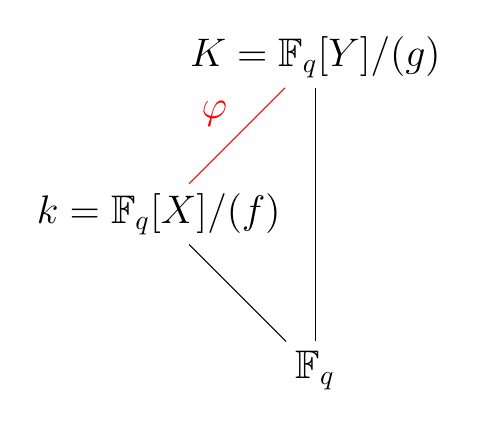
\begin{tikzpicture}[node distance=8em,font=\Large]
        \node(Fq){$\F_q$};
        \node(Fqf)[above left of=Fq]{$k=\F_q[X]/(f)$};
        \node(Fqg)[above right of=Fqf]{$K=\F_q[Y]/(g)$};
        \draw[]
        (Fq) edge (Fqf)
        (Fq) edge (Fqg)
        (Fqf) edge[left,auto,color=alert] node{$\varphi$} (Fqg);
      \end{tikzpicture}
    \end{wrapfigure}

    \paragraph{Let}
    \begin{itemize}
    \item $\F_q$ be a field with $q$ elements,
    \item $f$ and $g$ be irreducible polynomials in $\F_q[X]$ and
      $\F_q[Y]$,
    \item $m=\deg f$, $n=\deg g$ and $m|n$.
    \end{itemize}

    There exists a field
    embedding \[\color{alert}\varphi:k\hookrightarrow K,\] unique up to
    \mbox{$\F_q$-auto}morphisms of $k$.

    \paragraph{Goals}
    \begin{itemize}
    \item \textbf{Represent} $\varphi$ efficiently,
    \item \textbf{Evaluate/Invert} $\varphi$ efficiently,
    \end{itemize}

    When $\deg f = \deg g$, this is also called the
    \emph{isomorphism problem}. 
    
    \paragraph{Applications}
    \begin{itemize}
    \item Fundamental building blocks of computer algebra systems.
    \item Work algorithmically in the algebraic closure
      $\bar{\F}_q$~\cite{bosma+cannon+steel97}.
    \end{itemize}
  }

  \block{Embedding description}{ 
    \begin{wrapfigure}[8]{r}{0.4\colwidth}
      \centering
      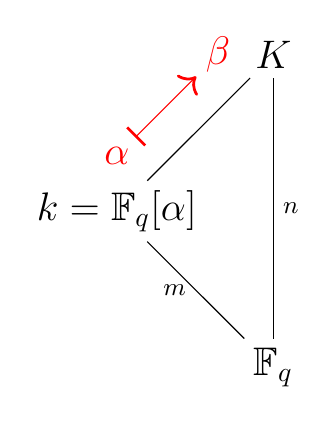
\begin{tikzpicture}[node distance=8em,font=\Large]
        \node(Fq){$\F_q$};
        \node(Fqf)[above left of=Fq]{$k=\F_q[\alpha]$};
        \node(Fqg)[above right of=Fqf]{$K$};
        \begin{scope}[alert,node distance=2em]
          \node(a)[above of=Fqf]{$\alpha$};
          \node(b)[left of=Fqg]{$\beta$};
        \end{scope}
        \draw[auto,font=\small]
        (Fq) edge node[left]{$m$} (Fqf)
        (Fq) edge node[right]{$n$} (Fqg)
        (Fqf) edge (Fqg);
        \draw[|->,alert]
        (a) edge (b);
      \end{tikzpicture}
    \end{wrapfigure}

    \textbf{Determine} elements $\alpha\in k$ and $\beta\in K$ such
    that

    \begin{itemize}
    \item $\alpha$ generates $k=\F_q[\alpha]$,
    \item there exists $\varphi:\alpha\mapsto\beta$.
    \end{itemize}

    \paragraph{Naive solution:} take
    \begin{itemize}
    \item $\alpha= X \mod f(X)$, and
    \item $\beta$ a root of $f$ in $K$.
    \end{itemize}
    Cost of factorization: $\tildO(mn)$.\\ Storage: $O(n)$.

    \paragraph{Kummer-type algorithms}: Use properties of $m$-th
      roots of unity.
    \paragraph{Group-based algorithms}: Use properties of an
      algebraic group $G/\F_q$.
  }

  \block{Embedding evaluation}{ 
    \begin{wrapfigure}[8]{r}{0.2\colwidth}
      \centering
      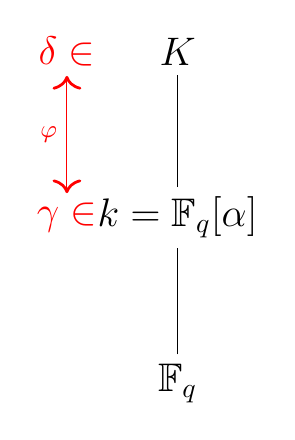
\begin{tikzpicture}[node distance=6em,font=\Large,on grid]
        \node(Fq){$\F_q$};
        \node(Fqf)[above=of Fq]{$k=\F_q[\alpha]$};
        \node(Fqg)[above=of Fqf]{$K$};
        \begin{scope}[alert,node distance=4em]
          \node(a)[left=of Fqf]{$\gamma\in$};
          \node(b)[left=of Fqg]{$\delta\in$};
        \end{scope}
        \draw
        (Fq) edge (Fqf)
        (Fqf) edge (Fqg);
        \draw[<->,alert]
        (a) edge node[left,auto,font=\small]{$\varphi$} (b);
      \end{tikzpicture}
    \end{wrapfigure}

    \textbf{Given}
    \begin{itemize}
    \item a \emph{description} of the embedding (as above),
    \item $\gamma\in k$ and $\delta\in K$,
    \end{itemize}

    \textbf{Solve} the following problems:
    \begin{itemize}
    \item Compute $\varphi(\gamma)$ in $K$.
    \item Test if $\delta\in\varphi(k)$.
    \item Supposing $\delta\in\varphi(k)$, compute $\varphi^{-1}(\delta)$ in $k$.
    \end{itemize}
    
    \textbf{Naive solution:} Linear algebra (size $n\times m$).
  }

  %%%%%%%%%%%%%%%%%
  % Kummer-type
  %%%%%%%%%%%%%%%%%
  \secblock{Kummer-type algorithms}

  \block{Lenstra's algorithm~\cite{LenstraJr91}}{
    \begin{wrapfigure}{l}{\colwidth}
      \paragraph{Goals}
      \begin{itemize}
      \item Prove that the isomorphism problem is \emph{deterministic
          polynomial}.
      \item Pervasive use of linear algebra.
      \item Does not prove precise complexity. Rough estimate:
        $\Omega(n^3)$.
      \end{itemize}
    \end{wrapfigure}

    \begin{wrapfigure}[4]{r}{0.45\colwidth}
      \hfill
      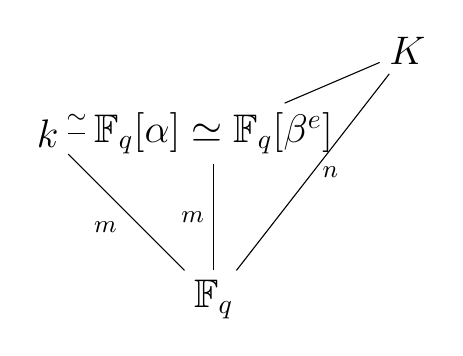
\begin{tikzpicture}[node distance=6em,font=\Large,on grid]
        \node(Fq){$\F_q$};
        \node(kum)[above=of Fq]{$\F_q[\alpha]\simeq\F_q[\beta^e]$};
        \node(k)[left=6em of kum]{$k$};
        \node(K)[above right=3em and 7em of kum]{$K$};
        \draw[auto,font=\small]
        (Fq) edge node{$m$} (kum)
        (Fq) edge node{$m$} (k)
        (Fq) edge node[right]{$n$} (K)
        (k) edge node[]{$\sim$} (kum)
        (kum) edge node{} (K);
      \end{tikzpicture}
    \end{wrapfigure}

    \paragraph{Technique}
    \begin{itemize}
    \item Reduce to $n$ a prime power.
    \item If $(n,q)>1$,
      \begin{itemize}
      \item  use Artin-Schreier theory.
      \end{itemize}
    \item Else, use Kummer theory:
      \begin{itemize}
      \item find $\alpha\in k$ s.t. $\alpha^m=a\in\F_q$,
      \item find $\beta\in K$ s.t. $\beta^m=b\in\F_q$,
      \item compute $a=b^e$, then $\alpha\mapsto\beta^e$.
      \end{itemize}
    \end{itemize}

    In general, if $m\nmid(q-1)$, adjoin roots of unity by working in
    \emph{cyclotomic extension rings}.
  
  }

  \column{0.333}
  \makeatletter
  \setlength{\TP@blockverticalspace}{10mm}
  \makeatother

  \block{Allombert's variant~\cite{Allombert02}}{
    \paragraph{Goals}
    \begin{itemize}
    \item Trade determinism for efficiency.
    \item Implementation integrated into Pari/GP.
    \item \textcolor{alert}{Still missing a rigorous complexity
        analysis. \Large\Sadey}
    \end{itemize}
    
    \paragraph{Technical differences}
    \begin{itemize}
    \item Allow factorization of cyclotomic polynomials to construct
      $\F_q[\mu_m]$.
    \item Explicit use of Hilbert 90 to compute $\alpha$ and
      $\beta$.
    \item $\alpha/\beta$ is in $\F_q[\mu_m]$: compute it by
      taking the $m$-th root of $a/b$.
    \item \textcolor{alert}{Use linear algebra to solve Hilbert
        90???}
    \item Use Shank's algorithm to compute $m$-th roots in
      $\F_q[\mu_m]$.
    \item \textbf{Complexity:} $O\left(m^{\omega+1}\right)$ (dominated
      by Hilbert 90).
    \end{itemize}
  }

  \block{Our improvements}{
    \begin{itemize}
    \item Classic trick (also present in Lenstra) + \emph{iterated
        frobenius}~\cite{vzgathen+shoup92:journal} to solve Hilbert
      90 \textbf{efficiently}:
      \[\alpha = \sum_{i=0}^{m-1}\zeta^i\gamma^{\sigma^{-i}}\]
      for $\zeta\in\mu_m$, $\sigma\in\Gal(\F_q[\mu_m])$, and random
      $\gamma$.
    \item Use factorization~\cite{kaltofen+shoup97} to compute $m$-th
      roots in $\F_q[\mu_m]$.
    \item \textcolor{alert}{Complexity analysis. \Large\Smiley}
    \item \textbf{Complexity:} $\tildO(m^2)$, but very efficient when
      $m\mid(q-1)$.
    \end{itemize}
  }

  %%%%%%%%%%%%%%%%%
  % Group-based
  %%%%%%%%%%%%%%%%%
  \secblock{Group-based algorithms}

  \block{Pinch's algorithm~\cite{Pinch}}{
    \begin{wrapfigure}[5]{r}{0pt}
      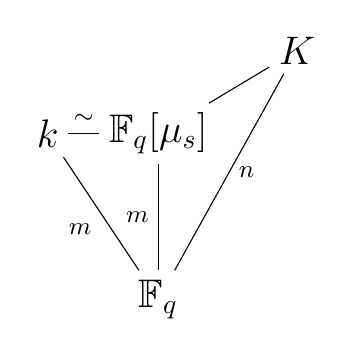
\begin{tikzpicture}[node distance=6em,font=\Large,on grid]
        \node(Fq){$\F_q$};
        \node(kum)[above=of Fq]{$\F_q[\mu_s]$};
        \node(k)[left=4em of kum]{$k$};
        \node(K)[above right=3em and 5em of kum]{$K$};
        \draw[auto,font=\small]
        (Fq) edge node{$m$} (kum)
        (Fq) edge node{$m$} (k)
        (Fq) edge node[right]{$n$} (K)
        (k) edge node[]{$\sim$} (kum)
        (kum) edge node{} (K);
      \end{tikzpicture}
    \end{wrapfigure}

    \paragraph{Idea}
    \begin{itemize}
    \item Find \emph{small} $s$ s.t. $k\simeq\F_q[\mu_s]$,
    \item Pick $s$-th roots of unity $\alpha\in k$, $\beta\in K$,
    \item Find $e$ s.t. $\alpha\mapsto\beta^e$.
    \item No complexity analysis {\Large\Sadey}, fast if $s$
      \emph{small}.
    \end{itemize}

    \paragraph{Technical details}
    \begin{itemize}
    \item $s$ is the smallest integer s.t. $\ord_s(q)=m$. 
    \item \textbf{Problem:} generically $s\in O(q^m)$.
    \item Test if $\alpha\mapsto\beta^e$ by linear algebra.
    \item \textbf{Problem:} tests are expensive, possibly $O(s)$ of
      them.
    \end{itemize}
    
    \paragraph{Elliptic variant}
    \begin{itemize}
    \item Replace $\mu_s$ by an $s$-torsion subgroup of an elliptic
      curve.
    \item Possibly more choices for $s$, \emph{hopefully} $s\in O(m)$.
    \end{itemize}

  }
  
  \block{Rain's cyclotomic algorithm~\cite{rains2008}}{
    \begin{wrapfigure}{r}{0.5\colwidth}
      \hfill
      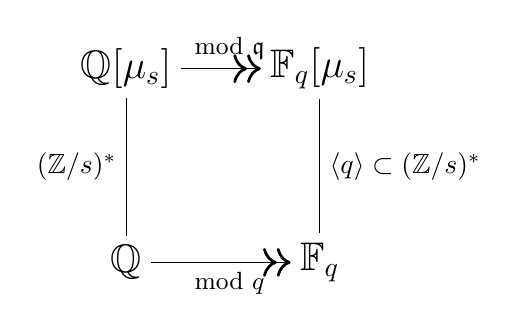
\begin{tikzpicture}[node distance=7em,font=\Large,on grid]
        \node(Fq){$\F_q$};
        \node(Q)[left=of Fq]{$\Q$};
        \node(k)[above=of Fq]{$\F_q[\mu_s]$};
        \node(C)[above=of Q]{$\Q[\mu_s]$};
        \draw[auto,font=\normalsize]
        (Fq) edge node[right]{$\langle q\rangle\subset(\Z/s)^\ast$} (k)
        (Q) edge node{$(\Z/s)^\ast$} (C);
        \draw[auto,font=\small,->>]
        (Q) edge node[below]{$\mod q$} (Fq)
        (C) edge node{$\mod\frak{q}$} (k);
      \end{tikzpicture}
    \end{wrapfigure}

    \paragraph{Removes trial-and-error}
    \begin{itemize}
    \item Replace $\alpha,\beta$ with \emph{Gaussian periods}:
      \[\eta(\alpha) = \sum_{\sigma\in S}\alpha^\sigma\]
      where $(\Z/s)^\ast = \langle q\rangle \times S$.
    \item Then $\eta(\alpha)\mapsto\eta(\beta)$.
    \end{itemize}

    \paragraph{Improves bound on $s$}
    \begin{itemize}
    \item Allow $\ord_s(q) = m\cdot o$, with small $o$,
      take degree $o$ extensions.
    \item Best bound: $s\in O(m^{2.4+\epsilon})$ (GRH), in practice
      $s\in O(m\log m)$.
    \item \textbf{Practical complexity:} $\tildO\left((mo)^2\log q\right)$. Fast
      when $o=1$.
    \end{itemize}

    \paragraph{Limitations}
    \begin{itemize}
    \item Unpublished. {\Large\Sadey} Implemented in Magma.
      {\Large\Smiley}
    \item Not really interesting for $q$ non-prime.
    \item Only practical for very small $o$.
    \end{itemize}
  }

  \column{0.333}
  \makeatletter
  \setlength{\TP@blockverticalspace}{14mm}
  \makeatother

  \block{Elliptic curve variant}{
    \begin{itemize}
    \item Replace Gaussian periods with \emph{elliptic
        periods}~\cite{mihailescu+morain+schost07}, $s$ an \emph{Elkies prime}.
    \item Same bounds on $s$: $O(m^{2.4+\epsilon})$ (GRH),
      $O(m\log m)$ (practical).
    \item \textbf{Practical complexity:} $\tildO\left(m\log q\right)$. 
    \item Slower than cyclotomic method for $o=1$, competitive
      otherwise.
    \item Works well with $q$ non-prime.
    \end{itemize}
  }

  %%%%%%%%%%%%%%%%%
  % Embedding evaluation
  %%%%%%%%%%%%%%%%%
  \secblock{Embedding evaluation}

  \block{Embedding evaluation and duality}{
    \begin{wrapfigure}[4]{r}{0.4\colwidth}
      \hfill
      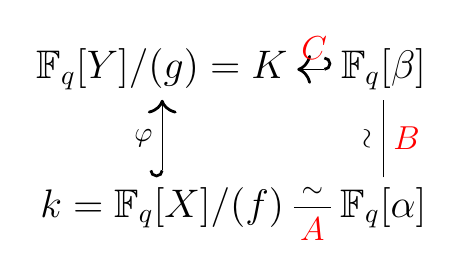
\begin{tikzpicture}[node distance=8em,font=\Large,on grid]
        \node(k)[]{$k=\F_q[X]/(f)$};
        \node(K)[above=5em of k]{$\F_q[Y]/(g)=K$};
        \node(Fqa)[right=of k]{$\F_q[\alpha]$};
        \node(Fqb)[right=of K]{$\F_q[\beta]$};
        \draw[auto,font=\normalsize]
        (k) edge node[above]{$\sim$} node[below,alert,font=\large]{$A$} (Fqa)
        (k) edge[c_->] node{$\varphi$} (K)
        (Fqa) edge node[rotate=90,above]{$\sim$} node[right,alert,font=\large]{$B$} (Fqb)
        (Fqb) edge[c^->] node[above,alert,font=\large]{$C$} (K);
      \end{tikzpicture}
    \end{wrapfigure}
    
    \paragraph{Evaluation decomposition}
    \begin{enumerate}
      \renewcommand{\labelenumi}{\textcolor{alert}{$\Alph{enumi}$.}}
    \item Dual of polynomial evaluation~\cite{shoup99}.
    \item Trivial.
    \item Evaluate polynomial in $\beta$ modulo $g$.
    \item[\color{alert}$\varphi^{\tiny-1}$.] Dual of
      \textcolor{alert}{$A\circ B\circ C$}
    \end{enumerate}

    \paragraph{Algorithms}
    \begin{itemize}
    \item Polynomial evaluation
      \begin{itemize}
      \item Horner's rule: $\tildO(mn)$,
      \item Modular composition: $O(n^{1+\epsilon})$~\cite{KeUm11},
        or $O(n^{(\omega+1)/2})$~\cite{brent+kung}.
      \end{itemize}
    \item Dual operations: same complexity as original (transposition
      principle).
    \end{itemize}
    
    \paragraph{Normal bases:}
    All the previous algorithms yield a \emph{normal element}
    $\alpha$.  Conversions to/from normal bases (\textcolor{alert}{$A,
      C$}) can be done in $O(n^{1.815}\log
    q)$~\cite{kaltofen+shoup98}.

  }

  \block[bodyinnersep=0]{Implementation}{
    \begin{itemize}
    \item C/Flint implementation of Allombert's algortihm,
    \item Sage/Cython implementation of Rains' and variants,
    \item Comparisons with Pari/GP, Sage, Magma, \dots
    \end{itemize}
    
    \begin{tikzpicture}[x=\colwidth/15,y=\colwidth/15]
      \draw (0,-0.4) [color=white,fill=white] rectangle (15,6.6);
      \node[inner sep=0,outer sep=0,anchor=south west]{\includegraphics[width=\colwidth]{bench}};
      \begin{scope}[line width=1pt,font=\small,anchor=east]
        \draw (6.5,2) node{naive}
        [Rays-Rays,color=red!70!black] -- (7.5,2);
        \draw (6.5,1.5) node{Allombert}
        [{Rays[n=8]}-{Rays[n=8]},color=blue!80!white] -- (7.5,1.5);
        \draw[line width=3pt] (6.5,1) node{elliptic Rains}
        [color=green!70!black] -- (7.5,1);

        \draw (13.5,2.4) node{$o=6$}
        [{Circle[open]-Circle[open]},color=red!70!black] -- (14.5,2.4);
        \draw (13.5,2.1) node{$o=4$}
        [Square-Square,color=cyan!50!white!] -- (14.5,2.1);
        \draw (13.5,1.8) node{$o=3$}
        [{Square[open]-Square[open]},color=magenta!80!blue] -- (14.5,1.8);
        \draw (13.5,1.5) node{$o=2$}
        [{Rays[n=8]}-{Rays[n=8]},color=blue!70!white] -- (14.5,1.5);
        \draw (13.5,1.1) node{elliptic}
        [line width=3pt,color=red!80!black] -- (14.5,1.1);
        \draw (13.5,0.8) node{$o=1$}
        [Rays-Rays,color=teal!70!green] -- (14.5,0.8);
      \end{scope}
      \begin{scope}
        \draw
        (0.2,3.2) node[font=\small,inner sep=0,rotate=90]{seconds}
        (4.3,0) node[font=\small]{degree $m$}
        (11.3,0) node[font=\small]{degree $m$}
        (1.2,5.3) node[anchor=west,font=\small]{$q=101$}
        (1.2,4.9) node[anchor=west,font=\small]{$m=n$}
        (8.2,5.3) node[anchor=west,font=\small]{$q=101$}
        (8.2,4.9) node[anchor=west,font=\small]{$m=n$}
        (4.3,6.2) node{comparison of main algorithms}
        (11.3,6.2) node{variants of Rains' algorithm};
      \end{scope}
    \end{tikzpicture}

    \begin{center}
      Code, data, notes and paper draft on
      \texttt{https://github.com/defeo/ffisom}
    \end{center}
  }

  \block{\refname}{
    \small
    \renewcommand*{\refname}{\vspace{-1em}}
    \bibliographystyle{plain}
    \bibliography{../defeo}
  }

\end{columns}

\end{document}